\documentclass[11pt, english, fleqn, DIV=15, headinclude]{scrartcl}

\usepackage[bibatend]{../header}
\usepackage{../my-boxes}

\usepackage{lastpage}
\usepackage{multicol}
\usepackage{simplewick}
\usepackage{multicol}
\usepackage{slashed}
\usepackage{subcaption}
\usepackage{cancel}
\usepackage{tikzsymbols}

\newcommand\timeorder{\mathscr T}
\newcommand\normorder{\mathscr N}
\newcommand\eye{\mat 1_4}
\newcommand\fourslash[1]{\slashed{\four{#1}}}
\newcommand\T{\mathrm T}

\hypersetup{
    pdftitle=
}

\graphicspath{{build/}}

\newcounter{totalpoints}
\newcommand\punkte[1]{#1\addtocounter{totalpoints}{#1}}

\newcounter{problemset}
\setcounter{problemset}{7}

\subject{physics7501 -- Advanced Quantum Field Theory}
\ihead{physics7501 -- Problem Set \arabic{problemset}}

\title{Problem Set \arabic{problemset}}

\newcommand\thegroup{Tutor: Thorsten Schimannek}

\publishers{\thegroup}
\ofoot{\thegroup}

\author{
    Martin Ueding \\ \small{\href{mailto:mu@martin-ueding.de}{mu@martin-ueding.de}}
}
\ifoot{Martin Ueding}

\ohead{\rightmark}

\begin{document}

\maketitle

\vspace{3ex}

\begin{center}
    \begin{tabular}{rrr}
        Problem & Achieved points & Possible points \\
        \midrule
        \nameref{homework:1} & & \punkte{15} \\
        \midrule
        Total & & \arabic{totalpoints}
    \end{tabular}
\end{center}

\vspace{3ex}

\begin{center}
    \begin{small}
        This document consists of \pageref{LastPage} pages.
    \end{small}
\end{center}

\section{You can't say \enquote{functional} without \enquote{fun}}
\label{homework:1}

\subsection{Interaction}

In general we have
\[
    W(J) = \frac 12 \int \dif^4 x \dif^4 y \, J(\four x) D_\text F(\four x -
    \four y) J(\four y) \,.
\]
The $J(x)$ consists of two summands, therefore $W(J)$ consists of four
summands. We will focus on one off-diagonal summand here.
\begin{align*}
    W_{12}(J)
    &= \frac 12 \int \dif^4 x \dif^4 y \, \delta^{(3)}(\vec x - \vec x_1) D_\text F(\four
    x - \four y)
    \delta^{(3)}(\vec y - \vec x_2) \,.
    \intertext{%
        The spatial integrations will fix $\vec x$ and $\vec y$, $x^0$ and
        $y^0$ are still free and have to be integrated over. Splitting up the
        temporal and spatial arguments in the propagator, we have
    }
    &= \frac 12 \int \dif x^0 \dif y^0 \, D_\text F(x^0 - y^0, \vec x - \vec y)
    \,.
    \intertext{%
        Then we can insert the scalar propagator and obtain
    }
    &= \frac 12 \int \dif x^0 \dif y^0 \frac{\dif^4 p}{[2\piup]^4}
    \frac\iup{p^2 - m^2 + \iup \epsilon} \exp(- \iup p^0 [x^0 - y^0]) \exp(\iup
    \vec p \cdot [\vec x - \vec y])
    \,.
    \intertext{%
        The time integration probably is in an interval of length $T$. So we
        write the time integration to the end and make the limits explicit.
    }
    &= \frac 12
    \frac{\dif^4 p}{[2\piup]^4}
    \frac\iup{p^2 - m^2 + \iup \epsilon}
    \exp(\iup \vec p \cdot [\vec x - \vec y])
    \int_{t}^{t+T} \dif x^0 \int_{t}^{t+T} \dif y^0
    \exp(- \iup p^0 [x^0 - y^0])
    \intertext{%
        This is not handy, so we introduce new variables, $a := x^0 - y^0$ and
        $b := x^0 + y^0$. The Jacobi matrix of the inverse transformation is
        \[
            \pd{(x, y)}{(a, b)} = \frac12
            \begin{pmatrix}
                1 & 1 \\ -1 & 1
            \end{pmatrix} \,.
        \]
        The determinant of this matrix is $1/2$ as common factors of a matrix
        enter the determinant to the power $n$ where $n^2$ is the number of
        matrix elements. The change of variables in the integration is a
        pullback, therefore the Jacobian of the inverse transformation has to
        be used. The new integral therefore is
    }
    &= \frac 14
    \frac{\dif^4 p}{[2\piup]^4}
    \frac\iup{p^2 - m^2 + \iup \epsilon}
    \exp(\iup \vec p \cdot [\vec x - \vec y])
    \int \dif a \int \dif b
    \exp(- \iup p^0 a)
    \,.
\end{align*}
Before thinking about the new integration domain too hard, we note that
the integration over $a$ looks like it could give a $\delta(-p^0)$ term
if the integration was not bounded. Then a change in variables would give
another minus sign (which we need) and set the remaining $p^0$ in the
denominator to zero. The remaining $\int \dif b$ would have to give a factor of
$4T$ to give the desired result. Since the integration over $a$ is bounded,
there is no real $\delta(-p^0)$ emerging from that. The integration over $p^0$
cannot be used to give $\delta(-a)$ as there are other factors of $p^0$ in the
expression which alter the oscillatory behavior.

\subsection{Yukawa-potential}

\emph{Missing}

\subsection{Degrees of polarization}

We start off with the well known fact that
\begin{align*}
    - \eta_{\mu\nu} &= - \eta_{\mu\nu} \,.
    \intertext{%
        Then we can write the left side a tad more complicated by introducing
        more dummy indices. The idea is that only the diagonal elements of the
        metric tensor of special relativity are nonzero. Therefore we can write
        all those four nonzero elements explicitly as
    }
    - \delta^0_\mu \delta^0_\nu + \sum_{a} \delta^a_\mu \delta^a_\nu
    &= - \eta_{\mu\nu} \,.
    \intertext{%
        The Latin index $a$ runs over the numbers in the set $\{1, 2, 3\}$.
        Next we can move the first summand over to the other side. Our
        bootstrapped relation then is
    }
    \sum_{a} \delta^a_\mu \delta^a_\nu
    &= - \eta_{\mu\nu} + \delta^0_\mu \delta^0_\nu \,.
    \intertext{%
        On the left side we introduce the polarization basis vectors
        $\epsilon_\mu^a = \delta^a_\mu$. On the right side we write the
        Kronecker symbols at components of $\tilde{\four k} = (m, 0, 0, 0)$
        which is the momentum four-vector of a particle at rest. To do so, we
        have to divide by $m^2$ in order to remove the factor of $m$ that
        $\tilde{\four k}$ introduces. This procedure then takes us to
    }
    \sum_{a} \epsilon^a_\mu \epsilon^a_\nu
    &= - \eta_{\mu\nu} + \frac{\tilde k_\mu \tilde k_\nu}{m^2} \,.
    \intertext{%
        This is still in the rest frame of the particle in question. We need to
        boost it with a boost matrix~$\mat\Lambda$. All the index are lowered,
        so actually one would need the inverse transformation. Since one could
        just choose the rapidity with opposite sign we will not really bother
        with all the inverses here. Either way, we now boost everything to
        momentum $\four k$.
    }
    \Lambda_\mu{}^\alpha \Lambda^\nu{}_\beta \sum_{a} \epsilon^a_\alpha
    \epsilon^a_\beta
    &= - \Lambda_\mu{}^\alpha \Lambda_\nu{}^\beta \eta_{\alpha\beta} +
    \frac{\Lambda_\mu{}^\alpha \Lambda_\nu{}^\beta \tilde k_\alpha \tilde
    k_\beta}{m^2} \,.
    \intertext{%
        We now define all those explicit boosts away. The polarization vectors
        are to be taken at the momentum $\four k$. The vector $\tilde{\four k}$
        becomes $\four k$ with the transformation. The metric tensor does not
        change under the Lorentz transformation. Since that is the defining
        property of a Lorentz transformation it is rather pointless to show
        that explicitly. We talked about the Penrose diagrammatic notation last
        week, so just for the sake of including it, we have done so. The
        diagram is shown in Figure~\ref{fig:02} with a short explanation of the
        notation in Figure~\ref{fig:01}. To get back to the formulas, we now
        have
    }
    \sum_a \epsilon_\mu^a(\four k) \epsilon_\nu^a(\four k)
    &= - \eta_{\mu\nu} + \frac{k_\mu k_\nu}{m^2} \,.
    \intertext{%
        Now one can factor out a minus sign and arrive at the desired equation:
    }
    \sum_a \epsilon_\mu^a(\four k) \epsilon_\nu^a(\four k)
    &= - \sbr{\eta_{\mu\nu} - \frac{k_\mu k_\nu}{m^2}} \,.
\end{align*}

\begin{figure}
    \centering
    \begin{subfigure}[c]{0.3\linewidth}
        \centering
        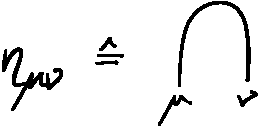
\includegraphics{Diagrams-page-01-crop.pdf}
        \caption{%
            Metric tensor
        }
        \label{fig:/1}
    \end{subfigure}
    \hfill
    \begin{subfigure}[c]{0.3\linewidth}
        \centering
        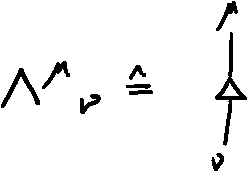
\includegraphics{Diagrams-page-03-crop.pdf}
        \caption{%
            Orthogonal transformation
        }
        \label{fig:/2}
    \end{subfigure}
    \hfill
    \begin{subfigure}[c]{0.3\linewidth}
        \centering
        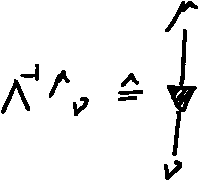
\includegraphics{Diagrams-page-04-crop.pdf}
        \caption{%
            Inverse transformation
        }
        \label{fig:/2}
    \end{subfigure}
    \caption{%
        Elements for the Penrose diagrammatic notation used in
        Figure~\ref{fig:02}.
    }
    \label{fig:01}
\end{figure}

\begin{figure}
    \centering
    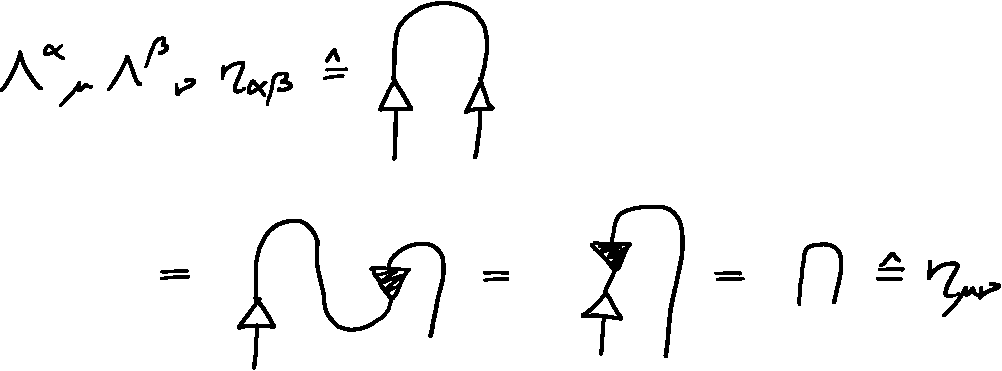
\includegraphics[width=\linewidth]{Diagrams-page-02-crop.pdf}
    \caption{%
        Showing that the metric tensor is not altered by a Lorentz
        transformation. In the first diagrammatic equality we have used that
        the transpose of the inverse is the matrix itself. Then we “wiggled”
        the paths to remove the two extra metric tensors in between to a
        Kronecker symbol. The matrix and the inverse are removed to give a
        Kronecker symbol as well. We end up with the metric tensor.
    }
    \label{fig:02}
\end{figure}

Writing it down in this way really makes clear where this extra $k_\mu k_\nu$
comes from. The sum over $a$ should really include $a = 0$, the temporal
polarization basis vector, as well. However, this is not a physical
polarization state, it needs to be subtracted. Also one can clearly see here
that this does not work as neatly with massless particles as there is no rest
frame for massless particles.

\subsection{Attraction of like charges}

\emph{Missing}

\subsection{Massive gravity}

A $4 \times 4$ tensor has 16 degrees of freedom. This means that the space
GL(4) has 16 generators or basis vectors. Their number is limited by a couple
constraints:

\begin{itemize}
    \item 
        First is the symmetry of the tensor. This removes six degrees of
        freedom, there are only ten left.

    \item
        The requirement that the basis tensors must not have any trace removes
        another degree of freedom.

    \item
        There is also some identity which looks like the Ward identity. A
        on-shell momentum four-vectors has three degrees of freedom. It would
        seem likely that the four equations (indexed by $\nu$) remove three
        degrees of freedom. The on-shell equation is another constraint as
        well, so all in all it removes four degrees of freedom.
\end{itemize}

The normalization of the basis vectors does not remove any degree of freedom in
the sense of a tensor space considered above. It only fixes the basis to some
particular value.

All in all we have $16 - 6 - 1 - 4 = 5$. So the number of basis elements
matches the number that we want to have.

The whole identity that we have to show can be boosted to the rest frame as all
the terms are $[4, 0]$-tensors and transform in the same way. Therefore it
suffices to look at the equation in the rest frame. There the tensor $\tens G$
takes the form
\[
    G_{\mu\nu}
    = \eta_{\mu\nu} - \frac{k_\mu k_\nu}{m^2}
    = \eta_{\mu\nu} - \delta_\mu^0 \delta_\nu^0
    \simeq
    \diag(0, -1, -1, -1)_{\mu\nu} \,.
\]

\subsection{Energy stress tensor}

So here we do not have $\tens G = 8 \piup G \tens T$ where the first
$\tens G$ is the Einstein tensor and the second $G$ is the gravitational
constant? Does the $\tens G$ from the problem here has any relation to the
Einstein tensor (except that it is symmetric)?

\end{document}

% vim: spell spelllang=en tw=79
